\chapter{Methods}

This chapter will introduce the relevant methodology used in this project. We will introduce two ways how to produce microdroplets, bulk microdroplets, where we used a magnetic stirrer to create microdroplets through rotation and on-chip microdroplets, where we used a microfluidic chip and pressured oil and water phases to create microdroplets. Then we will introduce halo-assays, a method to determine toxicity of antibiotics, used here to screen for potential target of antibiotic producers. Lastly, we will focus on liquid methodology which helped us to study the problems arising from our setup. We will introduce an experimental setup using conditional medium to study antibiotic production in liquid.

\section{Bulk droplets}
\label{sec:method_bulk_droplets}
Microdroplets can be produced in a flask using a magnetic stirrer and mixing an oil phase with a culture phase~(Figure~\ref{fig:method_droplet_experiments}a). To produce microdroplets in such a way, we mix 70ml of paraffin oil (with an added 2\% of AbilEM90, a surfactant used to guarantee stability of droplets over longer time) with 30ml of~\gls{LB} with added cultured bacteria. Mixing was performed by using a magnetic stirrer and slowly increasing the stirring speed up to a speed of 600~\gls{rpm}. We kept the stirring constant for 8 minutes before slowly reducing it again. 
\begin{figure}
\centering
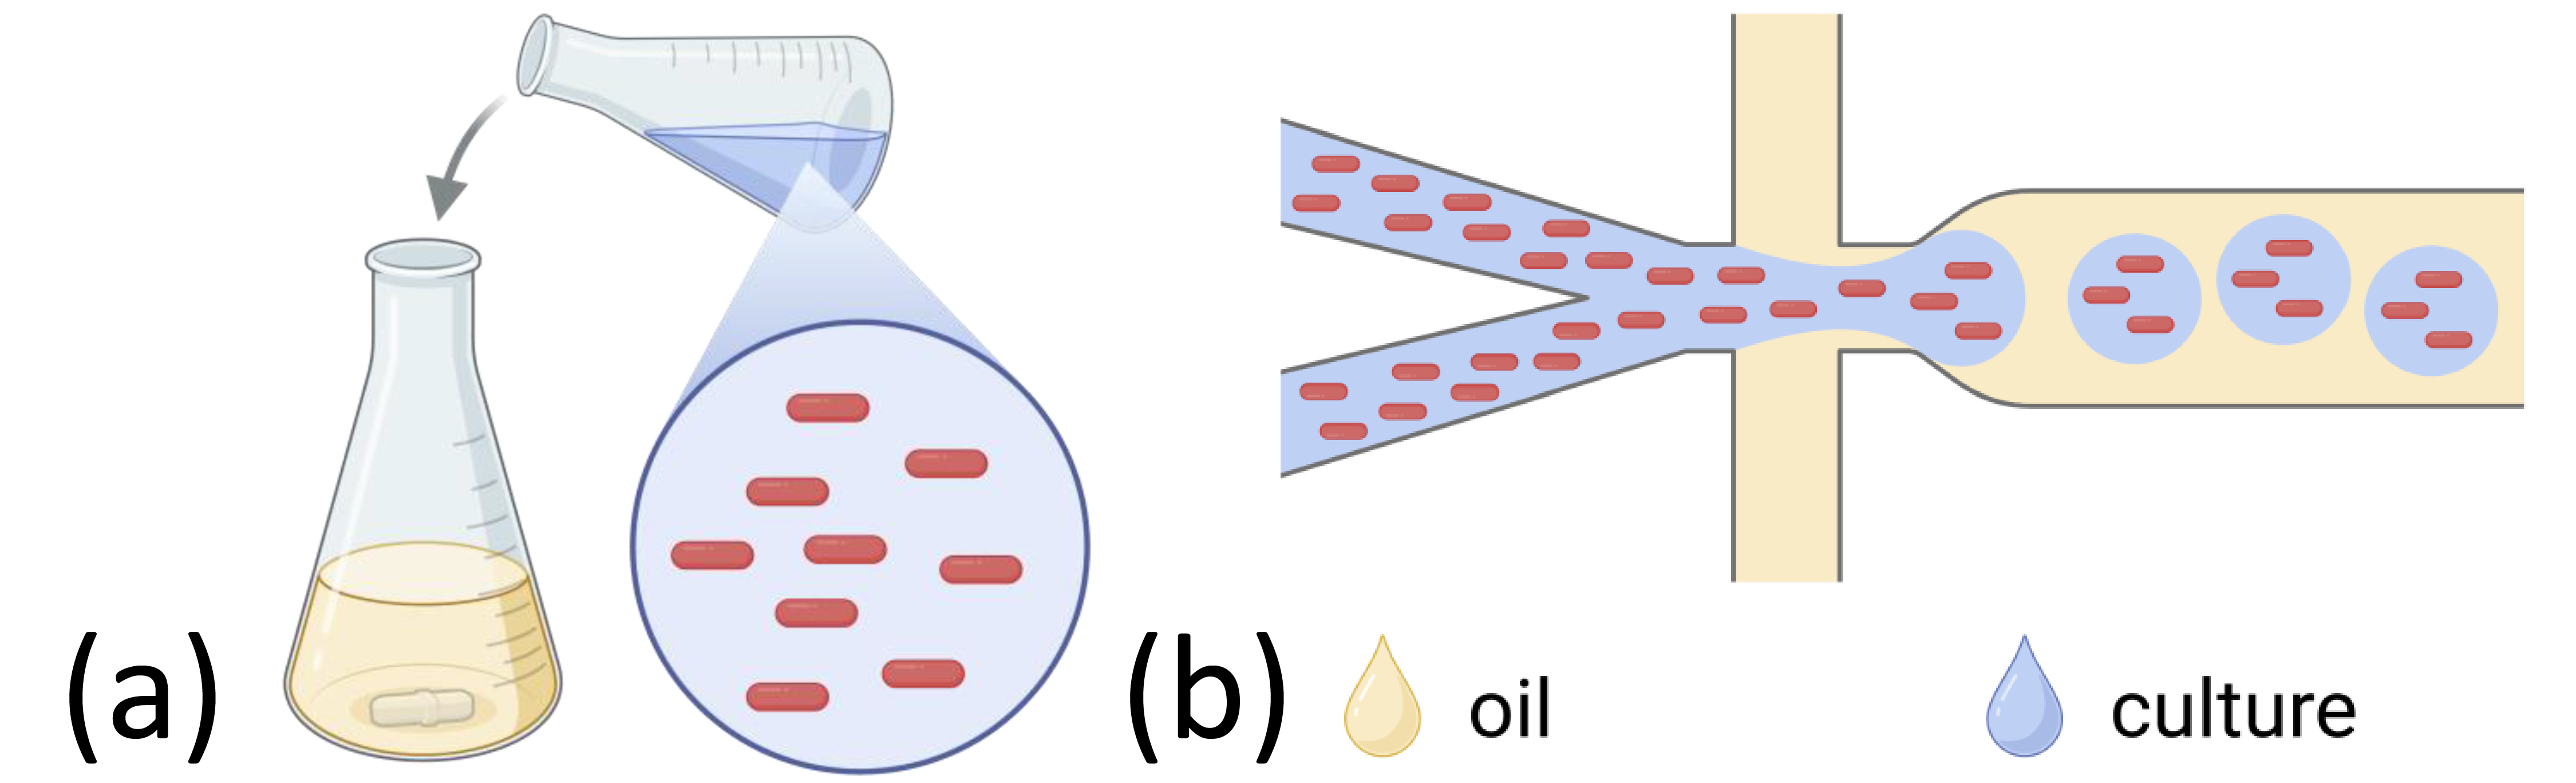
\includegraphics[width=\linewidth]{graphics/2025_09_30_droplets_fig2.png}
\caption{\textbf{Microdroplets can be produced using an in bulk method and using an on-chip method} (a) shows a sketch how to produce bulk microdroplets. In this method, an oil phase and a culture phase are mixed through stirring with a magnetic stirrer. (b) shows a sketch how to produce on-chip microdroplets. In this method, droplets are produced through pressurized oil and culture phases creating droplets at a junction inside the microfluidic chip.}
\label{fig:method_droplet_experiments}
\end{figure}

\section{On-chip droplets}
\label{sec:method_chip_droplets}
In this method, microdroplets were produced in a transparent, microfluidic chip. The chip has inlets through which pressurized oil and culture phases enter and flow to a junction. At the junction, these two phases form water-in-oil droplets which then flow into an outlet and from there in a collection vessel (Figure~\ref{fig:method_droplet_experiments}b). We used a commercially available 4-way microfluidic chip (Dolomite) to produce microdroplets and the same oil and surfactant in the chip as in bulk droplets but we also conducted experiments with Novec\textsuperscript{TM}7500 and added 0.5\% Pico-Surf{\textregistered} surfactant. This was recommended for usage with the specific chip we purchased.

\section{Halo assay}
\begin{figure}
\centering
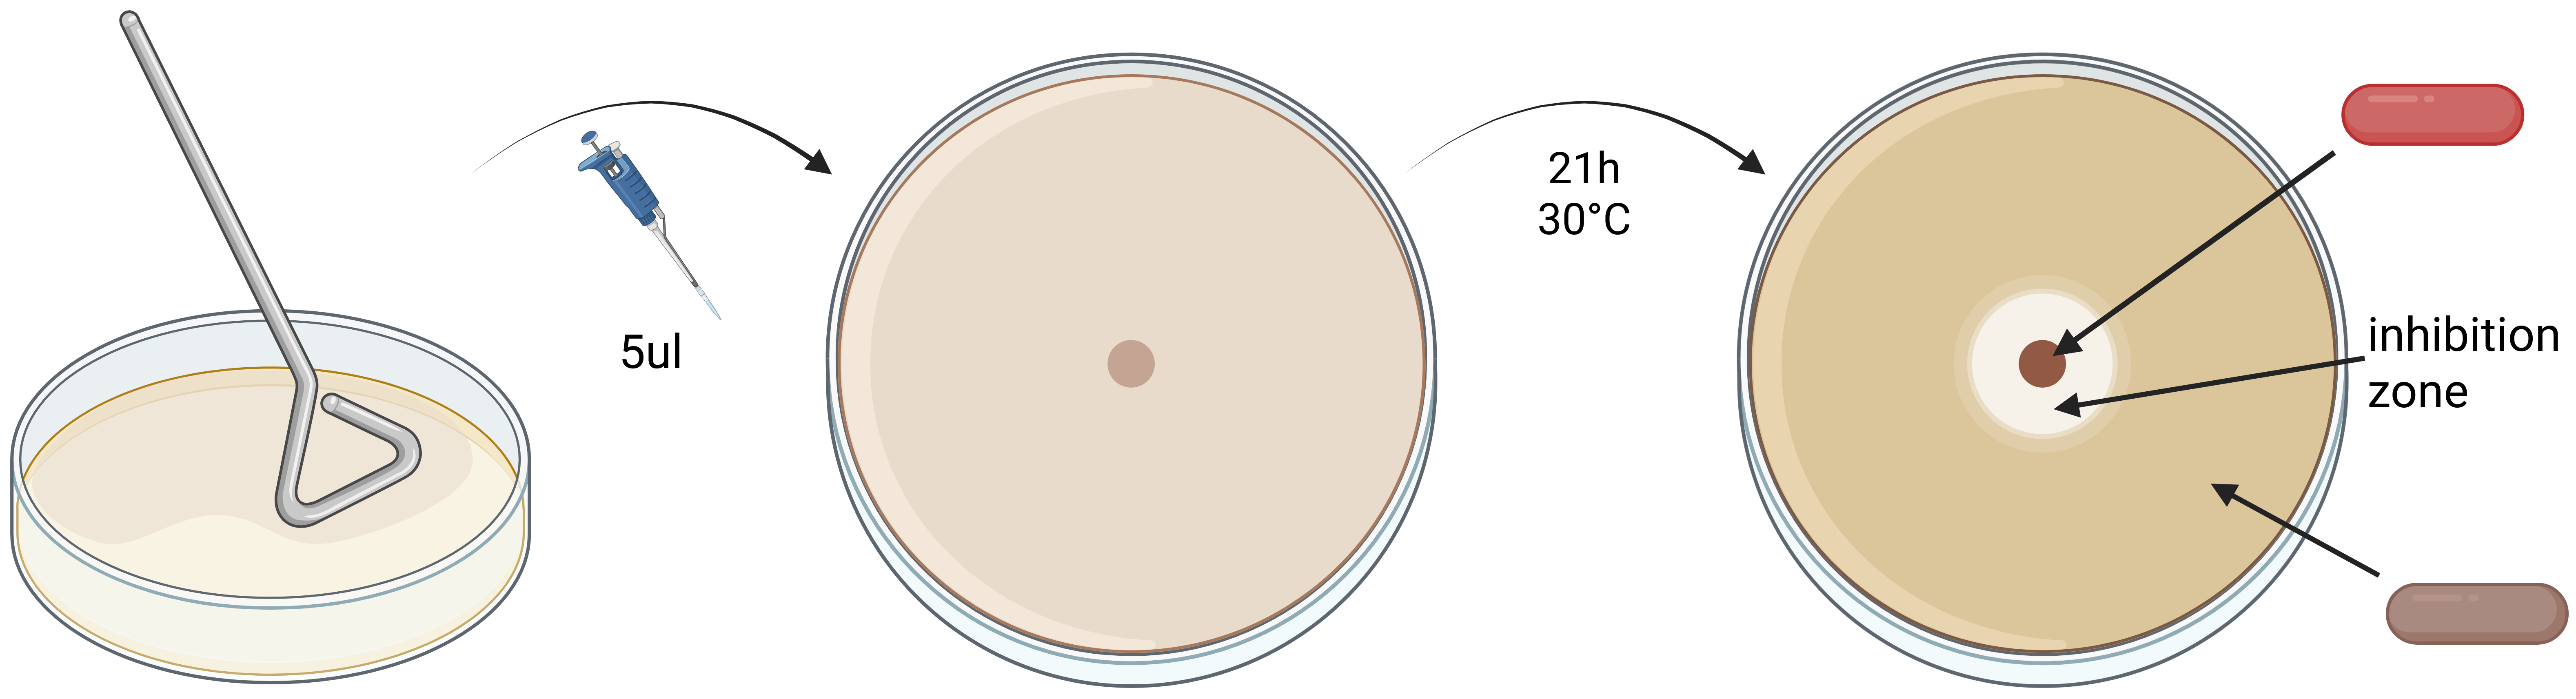
\includegraphics[width=\linewidth]{graphics/2025_09_30_droplets_fig3.png}
\caption{\textbf{Halo assays are used to test for antibiotic susceptibility} In a halo assay, first $100 \mu l$ of possible target bacteria (brown) were spread on an agar plate, then $5 \mu l$ of antibiotic producing bacteria (red) were spotted on top. After incubation for $21h$ at $30^\circ C$, the assay was evaluated. If the antibiotic is inhibiting growth, an inhibition zone was formed around the spot of antibiotic producer. The width of the zone indicates the effectiveness of the antibiotic against the target strain.}
\label{fig:method_halo_assay}
\end{figure}
We used halo assays to screen for possible target strains which are affected by produced antibiotics. In these assays, we spread $100\mu l$ of the target strain on an LB agar plate and then added drops of $5\mu l$ of the antibiotic producer on top of this. After $21h$ of incubation at $30^\circ C$, the target strain grew to a confluent lawn except if the antibiotic is toxic to the target. In that case, an inhibition zone around the drop of producing bacteria was formed. The width of the inhibition zone is a measure of effectivity of the antibiotic. A sketch of the assay is shown in Figure~\ref{fig:method_halo_assay}.

\section{Liquid and droplet comparison}
To understand how the growth conditions in standard liquid cultures and in microdroplets differ, we produced droplets and incubated both, droplets and the original culture phase in parallel. After droplet production, we determined the \gls{CFU} count of the initial culture and after $21h$ of incubation, we determined the \gls{CFU} count in both, droplets and liquid culture. We encapsulated antibiotic producer and target strain separately in distinct droplets to evaluate their growth in the absence of interactions.
\section{Conditional medium}
\begin{figure}
\centering
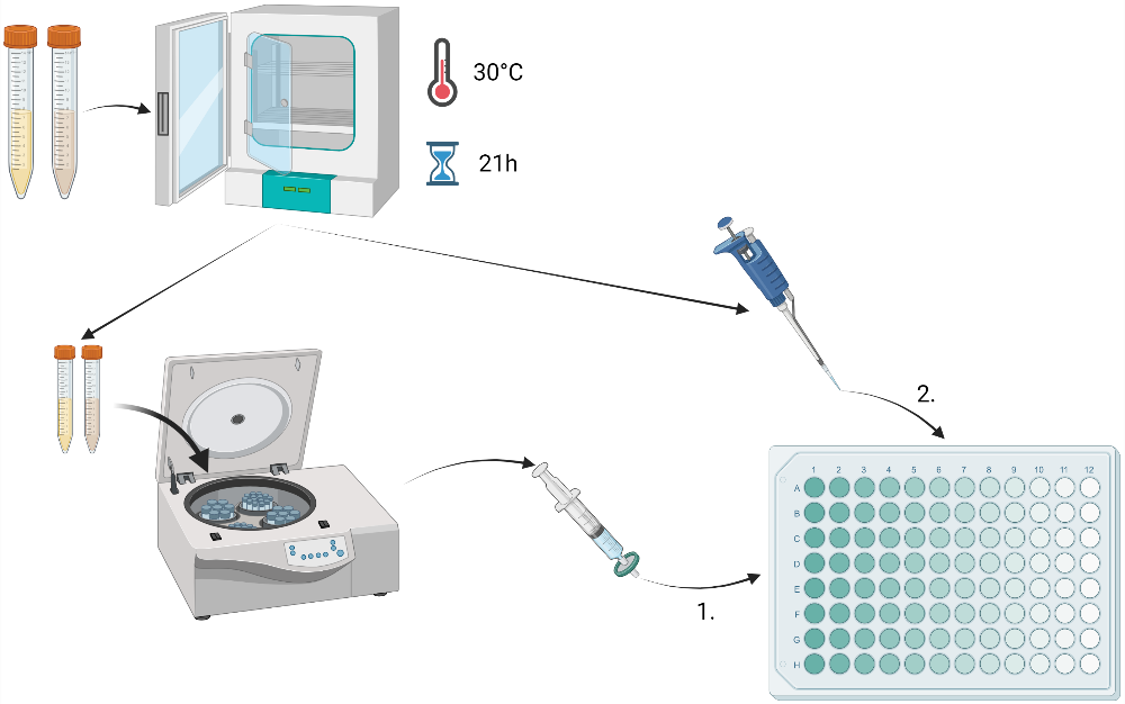
\includegraphics[width=\linewidth]{graphics/2025_09_30_droplets_fig4.png}
\caption{\textbf{A conditional medium assay can determine the efficiency of a produced antibiotic in liquid.} We used this assay to check for antibiotic production in liquid. In this method an overnight culture is centrifuged and filtered to remove bacteria and the remaining so called conditional medium was used to determine toxicity of produced antibiotics in this conditional medium on other bacteria. For this, a 2-fold dilution series was performed, with which we can measure interactions between bacteria, when growing a different strain in this conditional medium.}
\label{fig:method_conditional_medium}
\end{figure}
To measure the effect of produced antibiotics in growth medium on another bacterial strain, we used conditional medium. We inoculated bacteria in 10ml~\gls{LB} and grew these at $30^\circ C$ for 21h with shaking (200~\gls{rpm}). After incubation, we centrifuged half of the culture for 7 minutes at 3500~\gls{rpm}. Afterwards, the liquid was carefully filtered with a $0.45 \mu m$ filter. The filtered conditional medium was diluted in a 2-fold dilution series on a 96well plate with fresh medium. The initial culture was diluted 1:1000 in the prepared dilution series and grown at $30^\circ C$  with shaking (200~\gls{rpm}). OD600 was read out to measure growth. Using producer and target strain, we grew each one in its own conditional medium and in the respective other one. Figure~\ref{fig:method_conditional_medium} shows a sketch of the experimental protocol.